\documentclass{cshwk}

\title{Principles of Database Systems\\Assignment \#1 - Initial Report}

\begin{document}
\maketitle

\section{Downloading and Installing PostgreSQL}
Scence I am using \texttt{Arch Linux} as my primary operating system, I have installed \texttt{PostgreSQL} version \texttt{16.3-4} from the official repositories. Downloading and installing \texttt{PostgreSQL} on \texttt{Arch Linux} is as simple as running the following command:
\begin{verbatim}
    $ sudo pacman -S postgresql
\end{verbatim}
The result is shown in Fig.~\ref{fig:install}.
\begin{figure}[htbp]
    \centering
    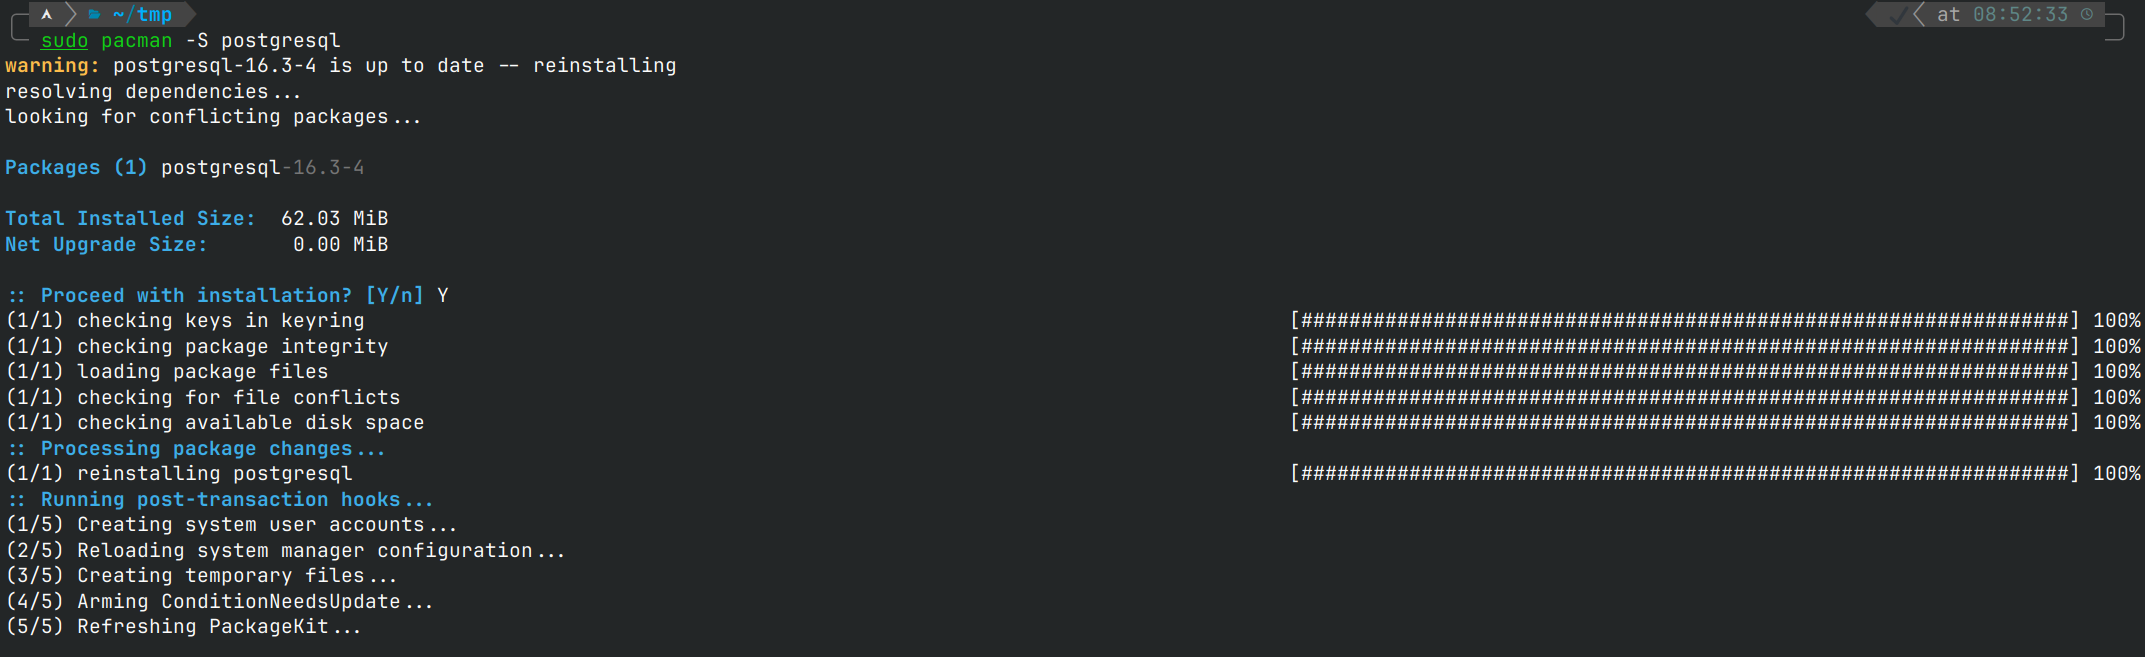
\includegraphics[width=0.8\textwidth]{hw1-1.png}
    \caption{Downloading and installing PostgreSQL on Arch Linux}
    \label{fig:install}
\end{figure}

\section{Running PostgreSQL}
After installing \texttt{PostgreSQL}, I started the \texttt{PostgreSQL} service by running the following command:
\begin{verbatim}
    $ sudo systemctl start postgresql
\end{verbatim}
The result is shown in Figure \ref{fig:start}.

\begin{figure}[htbp]
    \centering
    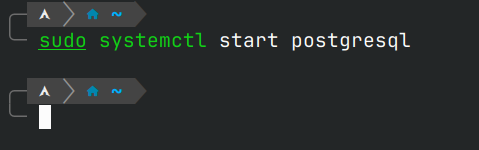
\includegraphics[width=0.5\textwidth]{hw1-2.png}
    \caption{Starting PostgreSQL service}
    \label{fig:start}
\end{figure}

\section{Trying to Connect to PostgreSQL}
I tried to connect to the \texttt{PostgreSQL} server by running the following command:
\begin{verbatim}
    $ psql -U postgres
\end{verbatim}

The -U option is used to specify the username for connecting to the server. The default username is postgres, which is the superuser for the PostgreSQL server. After connecting, use \textbackslash db to list all databases. The result is shown in Figure \ref{fig:connect}.

\begin{figure}[htbp]
    \centering
    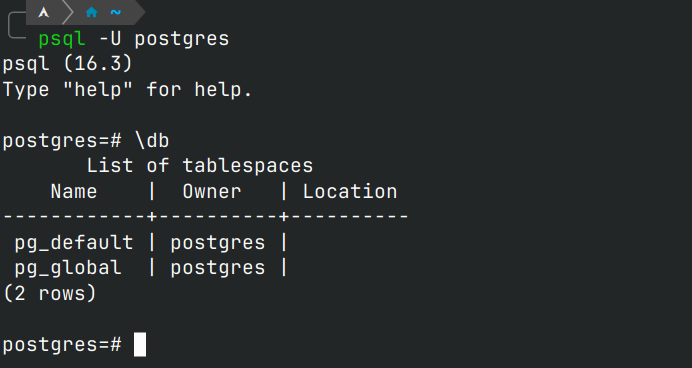
\includegraphics[width=0.8\textwidth]{hw1-3.png}
    \caption{Connecting to PostgreSQL server}
    \label{fig:connect}
\end{figure}

\end{document}